\chapter{評価}
\label{evaluation}

本章では,本システムが~\ref{issue:requirements}章で述べた課題解決における必要要件を満たしているか確認することで本研究の提案の評価を行う.
必要要件は以下の通りである.
\begin{itemize}
  \item OSやCPU, Memoryといったサーバ環境を柔軟に変更可能であること
  \item 公の実稼働環境を想定したネットワークでの通信の遅延を考慮できること
  \item 異なる管理権限下にある各サーバに対し統合的管理が可能であり,各オペレータの手作業を軽減できること
  \item 地理的に分散した各サーバに対し,統合的な操作が可能であること
\end{itemize}
評価では,本システムが地理的に分散したサーバに対して適用可能か,ならびに本システムを利用することによる手作業の削減の二点における定性評価,
加えてネットワーク上の遅延による本システムへの影響を定量的に評価した.

\section{地理的に分散したサーバに対する統合管理}

本システムでは,互いに疎通の取れない別セグメントをOpenVPNオーバーレイネットワークで繋ぎ,その上でKubernetesクラスタを構築した.
VPNによって異なるセグメントへの疎通性が確保されていることは,pingコマンドを用いて確認した.
以下は,Kubernetesクラスタ内のマスターノード(192.168.10.101)から別セグメントに配置されたワーカーノードに対してpingコマンドを実行した際の結果である.

\begin{lstlisting}[language=bash]
  $ ping 192.168.20.101 -c5
  PING 192.168.20.101 (192.168.20.101) 56(84) bytes of data.
  64 bytes from 192.168.20.101: icmp_seq=1 ttl=62 time=1.41 ms
  64 bytes from 192.168.20.101: icmp_seq=2 ttl=62 time=1.02 ms
  64 bytes from 192.168.20.101: icmp_seq=3 ttl=62 time=1.28 ms
  64 bytes from 192.168.20.101: icmp_seq=4 ttl=62 time=1.06 ms
  64 bytes from 192.168.20.101: icmp_seq=5 ttl=62 time=1.43 ms

  --- 192.168.20.101 ping statistics ---
  5 packets transmitted, 5 received, 0% packet loss, time 4005ms
  rtt min/avg/max/mdev = 1.028/1.243/1.432/0.172 ms
\end{lstlisting}

パケットロスはなく,通信が行えていることが確認できた.

次に,kubectlコマンドによって異なるセグメントに位置するサーバをクラスタリングできていることを確認した.

\begin{lstlisting}[language=bash]
  $ kubectl get nodes -owide
  NAME       STATUS     ROLES    VERSION   INTERNAL-IP       OS-IMAGE             KERNEL-VERSION      CONTAINER-RUNTIME
  master01   Ready      master   v1.16.3   192.168.10.101    Ubuntu 18.04.3 LTS   4.15.0-70-generic   docker://18.9.7
  master02   Ready      master   v1.16.3   192.168.10.102    Ubuntu 18.04.3 LTS   4.15.0-70-generic   docker://18.9.7
  master03   Ready      master   v1.16.3   192.168.10.103    Ubuntu 18.04.3 LTS   4.15.0-70-generic   docker://18.9.7
  node01     Ready      <none>   v1.16.3   192.168.20.101    Ubuntu 18.04.3 LTS   4.15.0-74-generic   docker://18.9.7
  node02     Ready      <none>   v1.16.3   192.168.20.102    Ubuntu 18.04.3 LTS   4.15.0-74-generic   docker://18.9.7
  node03     Ready      <none>   v1.16.3   192.168.30.101    Ubuntu 18.04.3 LTS   4.15.0-74-generic   docker://18.9.7
  node04     Ready      <none>   v1.16.3   192.168.30.102    Ubuntu 18.04.3 LTS   4.15.0-74-generic   docker://18.9.7
\end{lstlisting}

上記の結果から,異なるIPアドレスをもつサーバに対しクラスタリングを行えていることが確認できた.

最後に,Kubernetesクラスタ上にアプリケーションのデプロイが可能であるかを確認した.
NginxをKubernetesのワークロードであるDeploymentとしてクラスタ上にデプロイした結果が以下である.

\begin{lstlisting}[language=bash]
  $ kubectl create deployment --image nginx hello-world
  $ kubectl get pods -owide
  NAME                          READY   STATUS    RESTARTS   AGE     IP          NODE       NOMINATED NODE   READINESS GATES
  hello-world-c6c6778b4-5n74d   1/1     Running   0          4d22h   10.44.0.1   node01     <none>           <none>
  hello-world-c6c6778b4-6mrj4   1/1     Running   0          4d22h   10.42.0.1   node03     <none>           <none>
  hello-world-c6c6778b4-fmnxt   1/1     Running   0          4d22h   10.47.0.1   node02     <none>           <none>
  hello-world-c6c6778b4-r8b5w   1/1     Running   0          4d22h   10.44.0.2   node04     <none>           <none>
\end{lstlisting}

node01からnode04のすべてのワーカーノードに対してコンテナのデプロイが完了したことを確認できた.
これにより,異なるセグメントに位置するノードに対して統合管理が可能であることを確認した.

\section{オペレータの手作業の軽減}

本節では,本システムが異なる組織間での惑星規模の分散システムの試験においてオペレータの手作業を軽減可能であるか評価する.
複数の大学によって構成される研究ネットワークで,惑星規模の分散システムを試験する場合を考える.
試験に必要な作業を手作業で行った場合、以下の作業が必要であると考える。

\begin{enumerate}
  \item 各大学のリソース(OS, CPU, Memory)の共有
  \item 各大学における作業内容の確定・共有
  \item 各大学のサーバ管理者とのスケジューリングの調整
  \item 各大学でのデプロイ作業
  \item 各大学から作業完了の連絡が来るのを待機
  \item 全大学での作業完了の共有
  \item 試験環境の利用開始
\end{enumerate}

上記の作業は、試験環境に対する変更が必要になる度に行わなければならない。
手作業に加え、オペレータ間のコミュニケーションが密に求められる。
そのため、各オペレータが手作業で試験の準備をしなければいけないことによる時間の消費、属人性によるミスが発生する可能性がある。
対して本研究の提案システムを用いた場合、以下の作業のみで試験の準備を行える。

\begin{enumerate}
  \item Kubernetesの定義ファイルの作成
  \item kubectlコマンドによるコンテナの起動
\end{enumerate}

システムの統合管理が可能であるため、各オペレータの手作業を軽減することができることに加え、属人性を排除し作業の冪等性を担保することができる。

\section{通信の遅延による本システムへの影響}

本節では、通信の遅延による本システムへの影響をコンテナの起動時間を計測することによって定量評価した。
実験環境では、tcコマンドを用いて擬似的に通信の遅延を発生させた。
これによってマスターノードとワーカーノードの通信において100ms, 300ms, 500msの遅延を発生させ、
異なるコンテナ起動数においてすべてのワーカーノードでコンテナが起動するまでの時間を計測した。
計測にはkubectlコマンドのコンテナ監視機能を用いており、単位はこれに依存し秒(s)となっている。

\begin{figure}[htbp]
  \begin{center}
    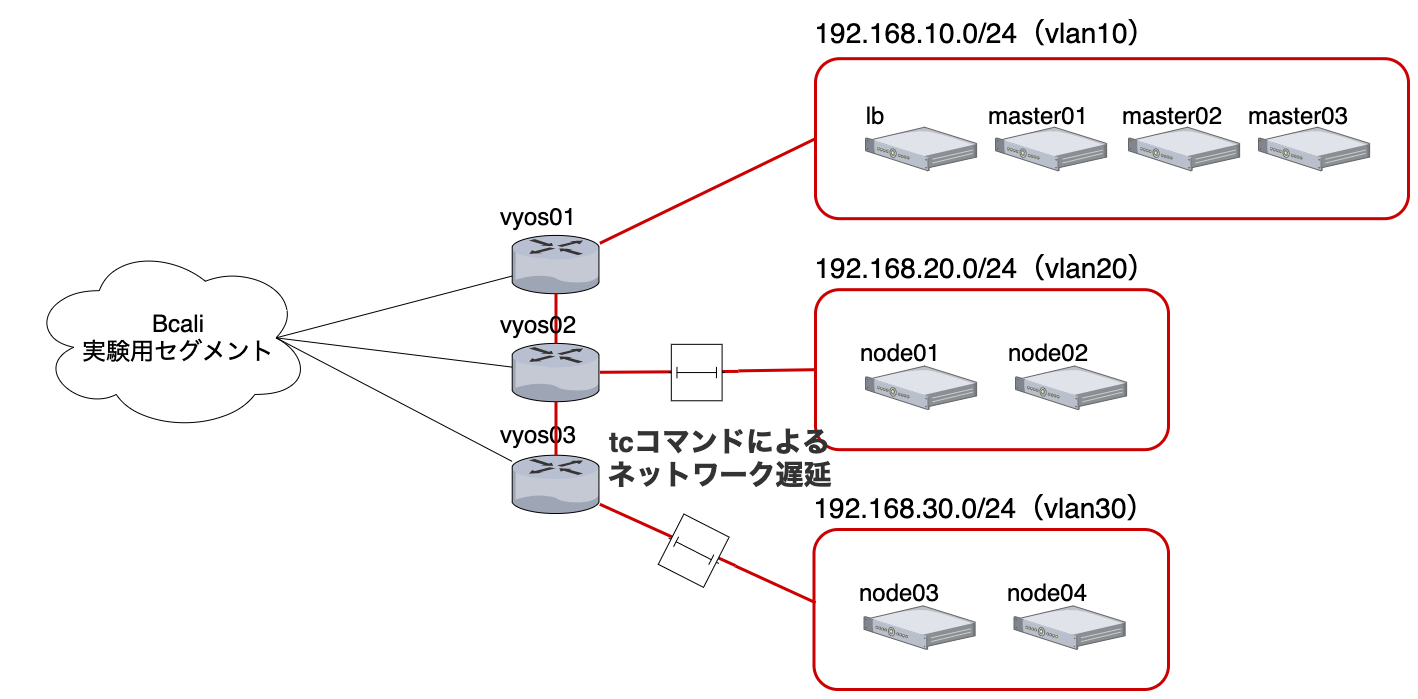
\includegraphics[width=0.4\textwidth]{./figures/tc.png}
    \caption{tcコマンドによるマスターノード・ワーカーノード間の擬似的な遅延の発生}
  \end{center}
\end{figure}



\section{評価のまとめ}

まとめ.

%%% Local Variables:
%%% mode: japanese-latex
%%% TeX-master: "./thesis"
%%% End:
